\documentclass[11pt]{report}
\usepackage{float}
\usepackage{graphicx}
\usepackage{fullpage}

\newcommand{\define}[2] {
  \textbf{Definition: #1}
  \begin{center} #2
\end{center}
}

\begin{document}

\title{PMR lecture notes}
\maketitle

\chapter{Prerequisites}

\section{Joint probability distribution}
A joint probability distribution is the PD of two random variables. This must sum to 1 as the probability of some combination must be 1.

If there are only two random variables, this is known as a bivariate distribution. If there are more than two variables this is known as a multivariate distribution. 

\subsection{Conditioning}
We can use conditioning as a means of reducing a joint probability distribution. However, the reduced version results in an normalised distribution which no longer sums to 1. 

\chapter{Belief networks}

A Bayes(or belief) network is a directed acyclic graph (DAG) whose nodes represent random variables $X_1...X_n$. For each node, $X_i$ has a CPD $P(X_i | Par_G(x_i))$ which denotes dependency on it's parent. Effectively, the BN represents a joint distribution via the chain rule.

\begin{figure}[H]
\centering
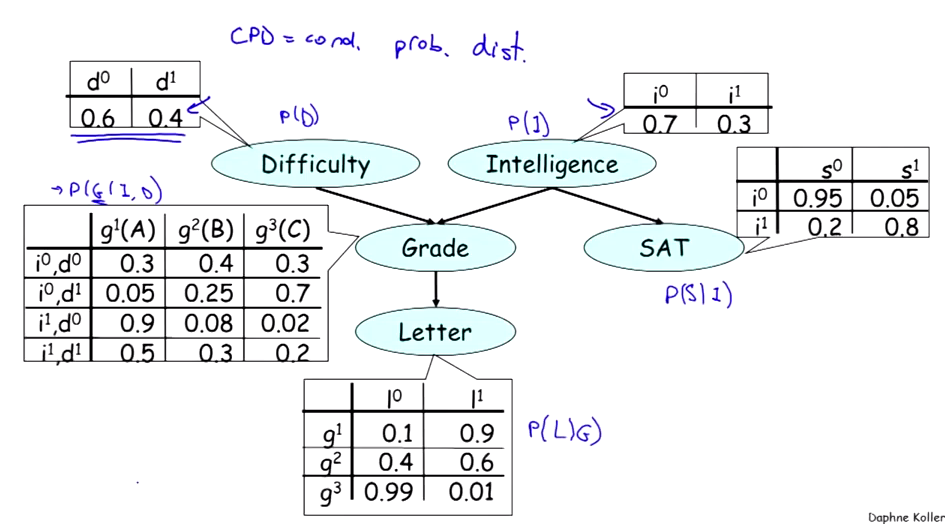
\includegraphics[scale=0.5]{images/cpd_bayesnetwork.png}
\caption{Bayes network with CPD details}
\label{belief1}
\end{figure}

This is an example of a Bayesian network. The nodes are dependent on each other as indicated by that arrows and the dependencies are the conditional probabilities. \\

But, how do we know that the Bayesian network is a legal distribution?

We need to show that the distribution is > 0. As P is a product of the CPD's and CPD's are non negative, they must always be bigger than zero.

Secondly, we need to prove that the distribution sums to 1. $\sum{P = 1}$

\define{Chain rule}{The chain rule takes all of the CPD's and multiplies them together}

\begin{figure}[H]
\centering
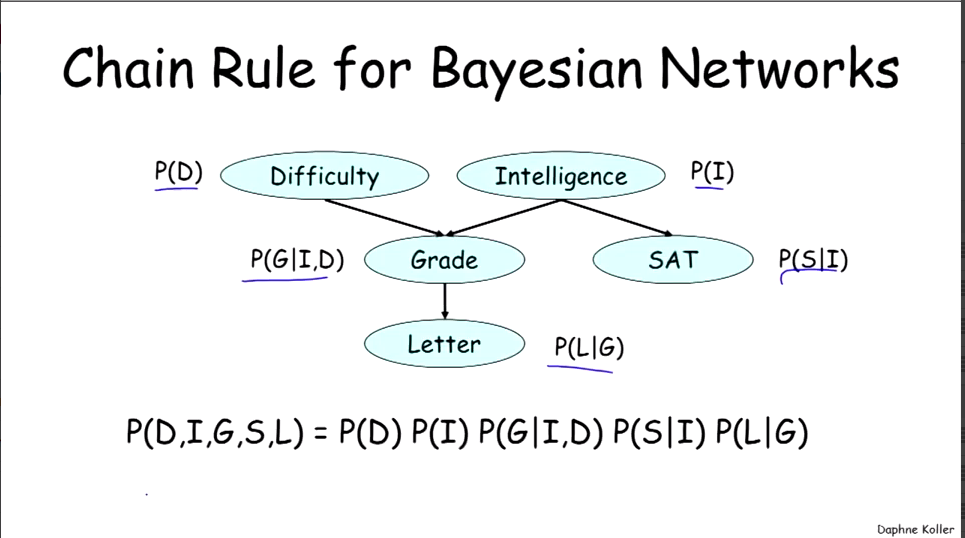
\includegraphics[scale=0.5]{images/cpd_chainrule.png}
\caption{Bayes network with higher level details of CPDs}
\label{sensorymockup2}
\end{figure}

\section{Questions}

\subsection{Question 1}
Given the Bayesian network in \ref{belief1}, what do you think is an appropriate factorization of the joint distribution P(D, I, G, S, L)?

Answer: P(D)P(I)P(G|I,D)P(S|I)P(L|G). This factorisation is also known as the chain rule. 

\subsection*{Question 2}
What is $P(d^0, i^1, g^3, s^1, l^1)$ in the Bayesian network \ref{belief1}?

Using the two images for information:

$i^1$ = 0.3 \\
$d^0$ = 0.6 \\
$l^1$ = 0.01 \\
$g^3$ = 0.02 - we look at the column for $g^3$ and find the row that corresponds to $d^0$ and $i^1$\\
$s^1$ = 0.8 \\

And we can multiply these together to get the answer. 


\chapter{Glossary}
\define{CPD}{Conditional probability distribution}
\define{Conditioning}{When we set one of the probabilities values (we condition it) as a means of reducing the network. See Coursera(Week 1, Distributions)}


\end{document}